\chapter{Vizualizácie}
\todo[inline]{cd priloha/web, spustenie, requirements, ...}

Cieľom tejto práce je nielen popísať \obliv pamäťový model a rôzne dátové štruktúry v ňom, ale aj vytvoriť ich vizualizácie. Tie majú slúžiť na edukačné účely pre študentov (a učiteľov) a pomáhať pri pochopení ich fungovania.

Výsledkom práce sú vizualizácie demonštrujúce dátové štruktúry popísané v predchádzajúcich sekciách: \vEB usporiadanie (sekcia \ref{sec:static-obliv}) v statickom binárnom vyhľadávacom strome, usporiadané pole (\ref{sec:orderedfile}) a dynamický b-strom (\ref{sec:dynamic-obliv}). Súčasťou je tiež simulácia \cache (sekcia \ref{sec:extmem}) s možnosťou voľby parametrov $B$ a $M$ - veľkosť bloku a celková veľkosť.

\todo[inline]{Existujuce? nic nie je...}

\section{Gnarley trees}
Tieto vizualizácie sú implementované ako rozšírenie programu \emph{Gnarley trees}, ktorý vznikol ako súčasť bakalárskej práca Jakuba Kováča \citep{algviskuko}. Tento nástroj na vizualizáciu (prevažne stromových) dátových štruktúr bol následne v bakalárskych prácach \citep{algviskotrlova, algvistomkovic, algvislukca} a ročníkových projektoch rozšírený o mnohé ďalšie dátové štruktúry a v súčastnosti podporuje desiatky štruktúr, ako napríklad červeno-čierne, sufixové a intervalové stromy, \emph{union-find}, haldy a mnohé ďalšie.

\subsection{Funkcionalita}
Program umožňuje užívateľom zobrazovať tieto štruktúry a manipulovať s nimi. Všetky operácie sú rozložené na malé, jednoduché kroky a každý je vysvetlený keď sa vykonáva. Je možné posúvať sa po krokoch dopredu ale aj vracať sa dozadu - história krokov je neobmedzená\todo{limit?} a teda sa dá kedykoľvek vrátiť až k počiatočnému stavu. Toto je dôležité pri experimentovaní s danou štruktúrou, kedy dve rôzne operácie (alebo jedna operácia s dvoma rôznymi parametrami) spôsobia rôzne správanie a výsledky. Užívateľ má takto možnosť jednoducho sa po vykonaní prvej operácie vrátiť do predošlého stavu a preskúmať správanie druhej z nich.

Celý program je taktiež dvojjazyčný - je možné prepnúť medzi angličtinou a slovenčinou, čo umožňuje širšie použitie týchto vizualizácií.

\subsection{Prehľad programu}
\begin{figure}
    \centering
    \resizebox{0.9\textwidth}{!}{%
        \begin{tikzpicture}

\node[anchor=south west,inner sep=0] (IMG) at (0,0) {\includegraphics[width=18cm]{\FiguresPath/screenshots/bmp_cobtree_menu_sk}};
\draw [thick, darkgray] (IMG.south west) rectangle (IMG.north east);

%\draw[draw=red,xstep=1,ystep=1] (0,0) grid (18,12);
%\foreach \x in {0,1,...,18} { \node [anchor=north] at (\x,0) {\x}; }
%\foreach \y in {0,1,...,12} { \node [anchor=east] at (0,\y) {\y}; }

\draw [thick, ->] (2, 12.5) node [anchor=west] {Výber dátovej štruktúry} to [in=90, out=180] (1, 11.75);
\draw [thick, ->] (3, 12) node [anchor=west] {Výber jazyka} to [in=90, out=180] (2.5, 11.75);

\draw [thick, ->] (10, 12.5) node [anchor=west] {Aktuálna dátová štruktúra} to [in=90, out=180] (9, 11.25);

\draw [thick, ->] (13, 12) node [anchor=west] {Popis vykonávanej akcie} to [in=90, out=180] (11, 9.5);

\draw [thick, decoration={brace, amplitude=10pt, 
	/tikz/postaction = {
		decoration = {
			markings,
			mark = at position 0.5 with \coordinate (CP);
		}, decorate
	}
}, decorate] (4.25, 1) -- (4.25, 2.5);
\draw [thick] (2.5, -0.5) node [anchor=east] {Ovládací panel} to [in=180, out=0](CP);

\draw [thick, ->] (7, -0.5) node [anchor=west] {Povolenie krokovania} to [in=270, out=180] (6.35, 1.15);

\draw [thick, decoration={brace, amplitude=10pt, mirror,
	/tikz/postaction = {
		decoration = {
			markings,
			mark = at position 0.5 with \coordinate (PN);
		}, decorate
	}
}, decorate] (10.65, 1.95) -- (13.7, 1.95);
\draw [thick] (13, -0.5) node [anchor=west] {Krokovanie dopredu / dozadu} to [in=270, out=180] (PN);

\end{tikzpicture}    
    }
    \caption{Užívateľské rozhranie počas operácie vkladania kľúča $10$ do dynamického \obliv B-stromu (sekcia \ref{sec:dynamic-obliv}).}
    \label{fig:exmem_model}
\end{figure}

\todo[inline]{prehlad (screenshot), panely, pouzivanie, ...}

\section{Statický strom}
Najjednoduchšou dátovou štruktúrou je statický vyhľadávací strom. Implementovali sme vytvorenie tohto stromu a jeho uloženie v pamäti. Je možné strom zväčšiť alebo zmenšiť podľa preferencii - ukážky stromov rôznych veľkostí sú na obrázku \ref{fig:ss_static_sizes}. Čísla vo vnútorných vrcholoch sú kľúče, čísla nad vrcholom určujú jeho pozíciu v pamäti. Obdĺžnik nad stromom reprezentuje uloženie tohto stromu v poli. Vnútorné čísla sú opäť kľúče, pričom sú zoradené podla svojich pozícii zľava (pozícia $1$) doprava.

\begin{figure}
    \centering
    \subtop[]{%
        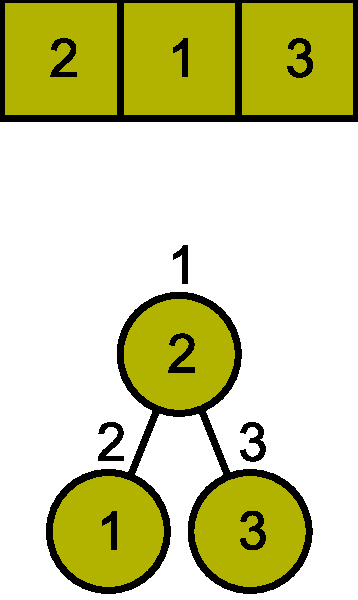
\includegraphics[scale=0.25]{figures/screenshots/static_size_2.pdf}}
    \subtop[]{%
        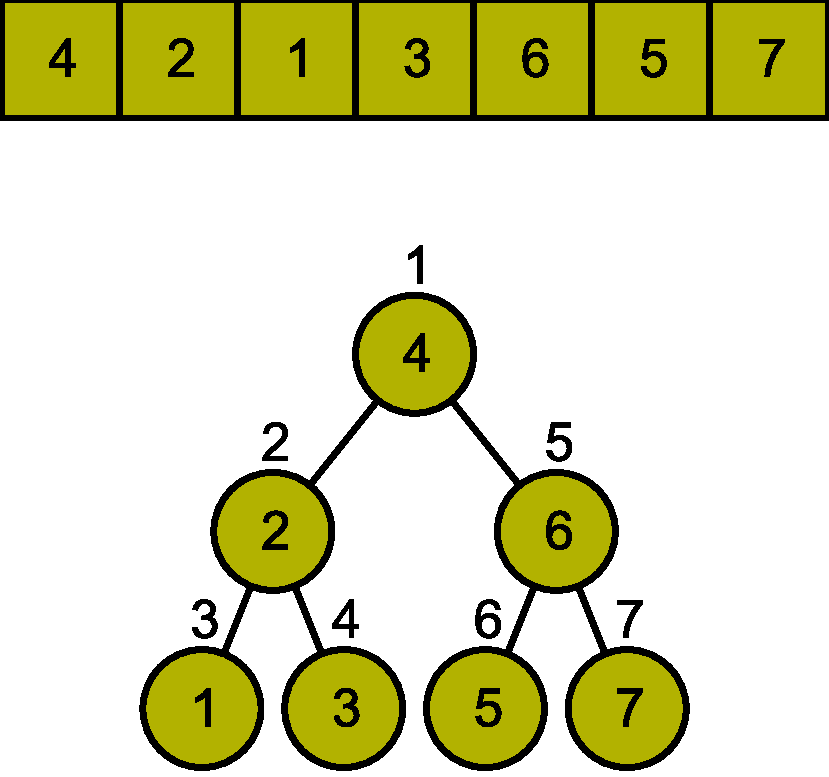
\includegraphics[scale=0.25]{figures/screenshots/static_size_3.pdf}}
    \subtop[]{%
        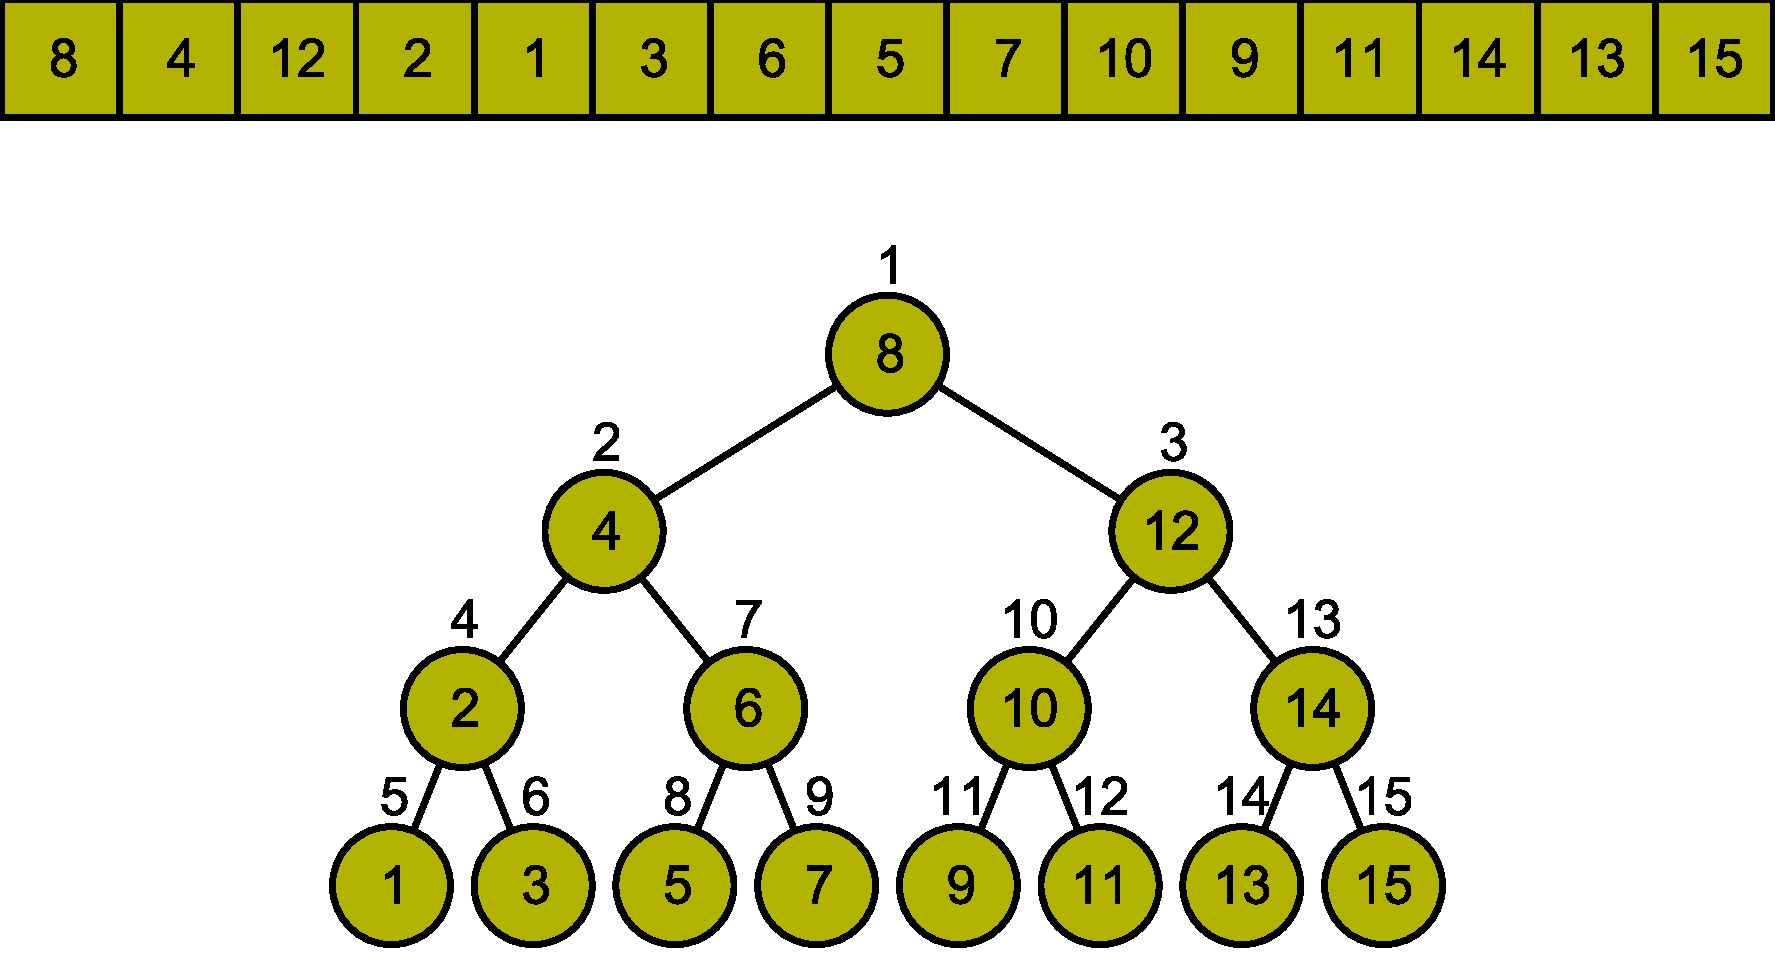
\includegraphics[scale=0.25]{figures/screenshots/static_size_4.pdf}}
    \caption{Statické stromy rôznych veľkostí (výšok) vo \vEB usporiadaní.}
    \label{fig:ss_static_sizes}
\end{figure}

Medzi uložením vo \vEB poradí a klasickom poradí (ako v časti \ref{sec:static-naive}) je možné prepínať. Zmenia sa pritom čísla udávajúce pozície vrcholov v pamäti a ich poradie v poli nad stromom. Rozdiel medzi týmito dvoma usporiadaniami vidieť na obrázku \ref{fig:ss_static_order}. Pozície sa zhodujú s obrázkom \ref{fig:node_order_comparison}.

\begin{figure}
    \centering
    \subtop[]{%
        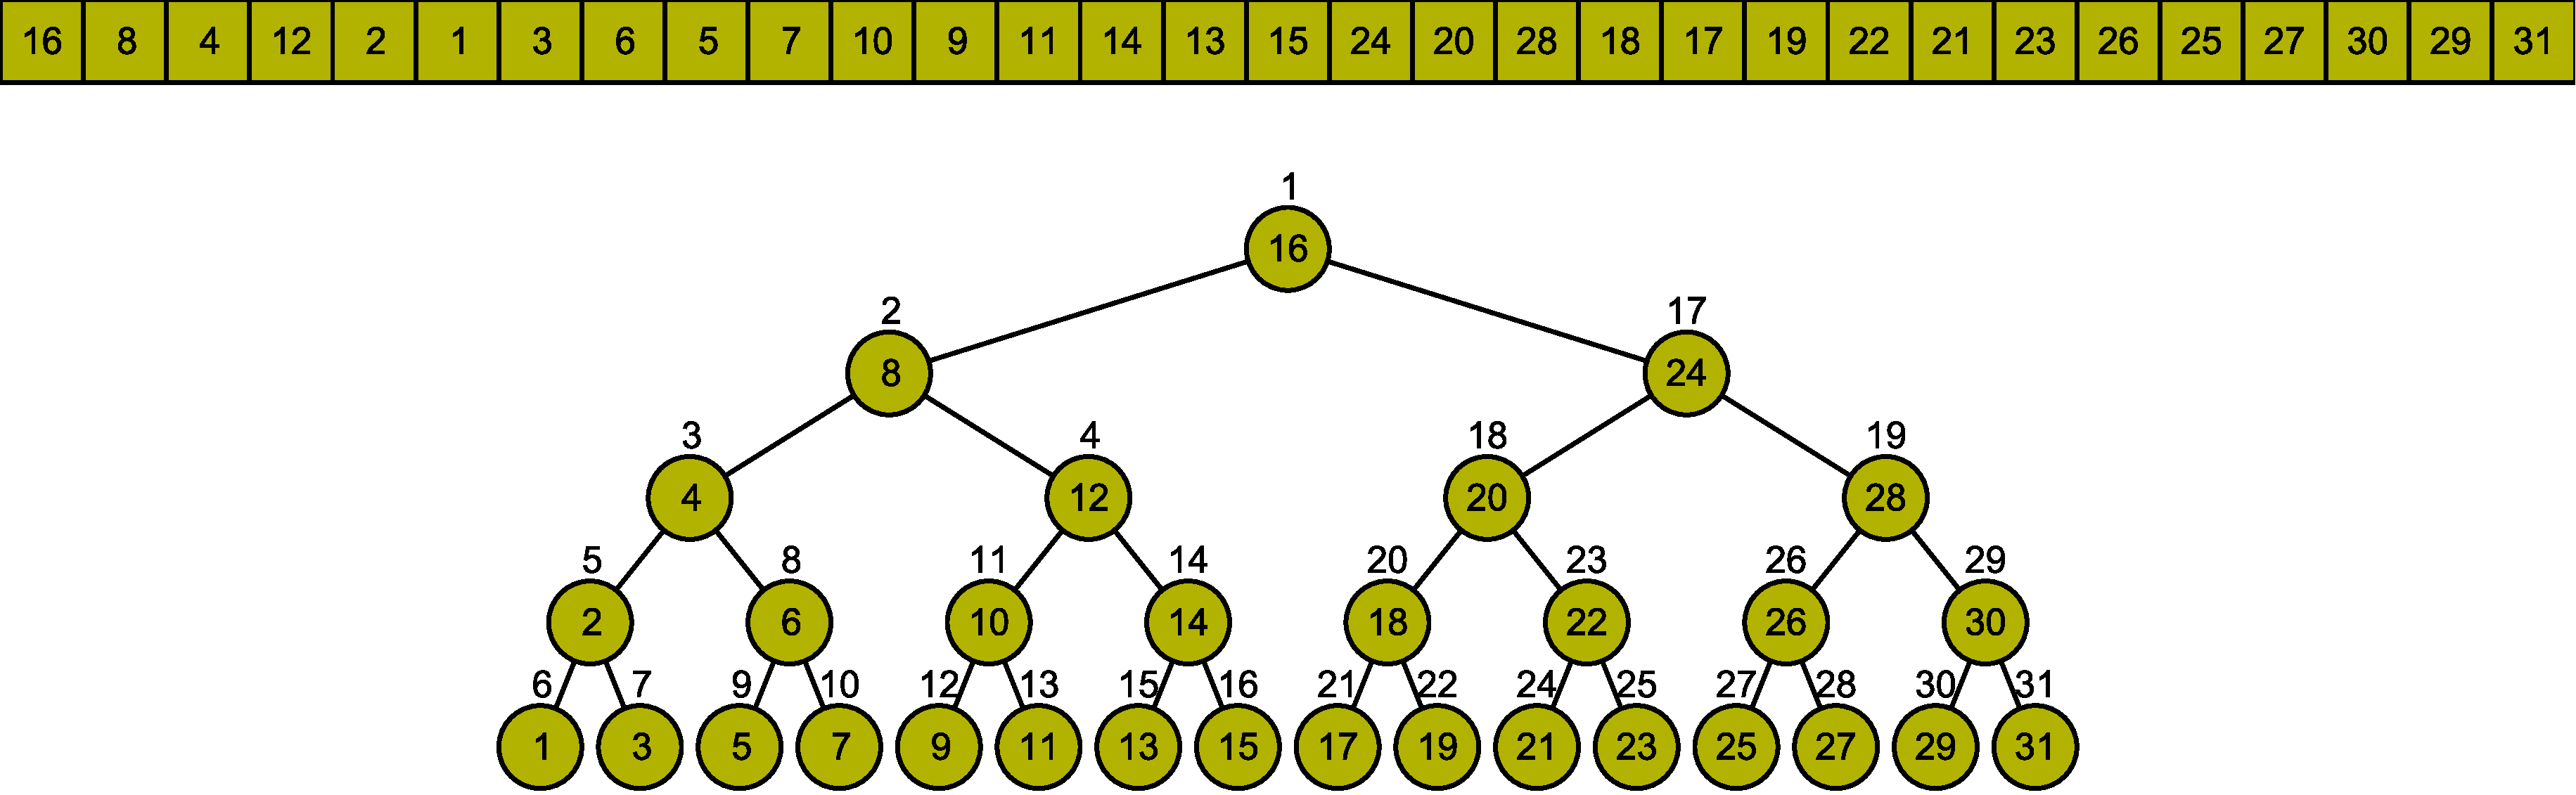
\includegraphics[width=\textwidth]{figures/screenshots/static_size_5.pdf}}
    \subtop[]{%
        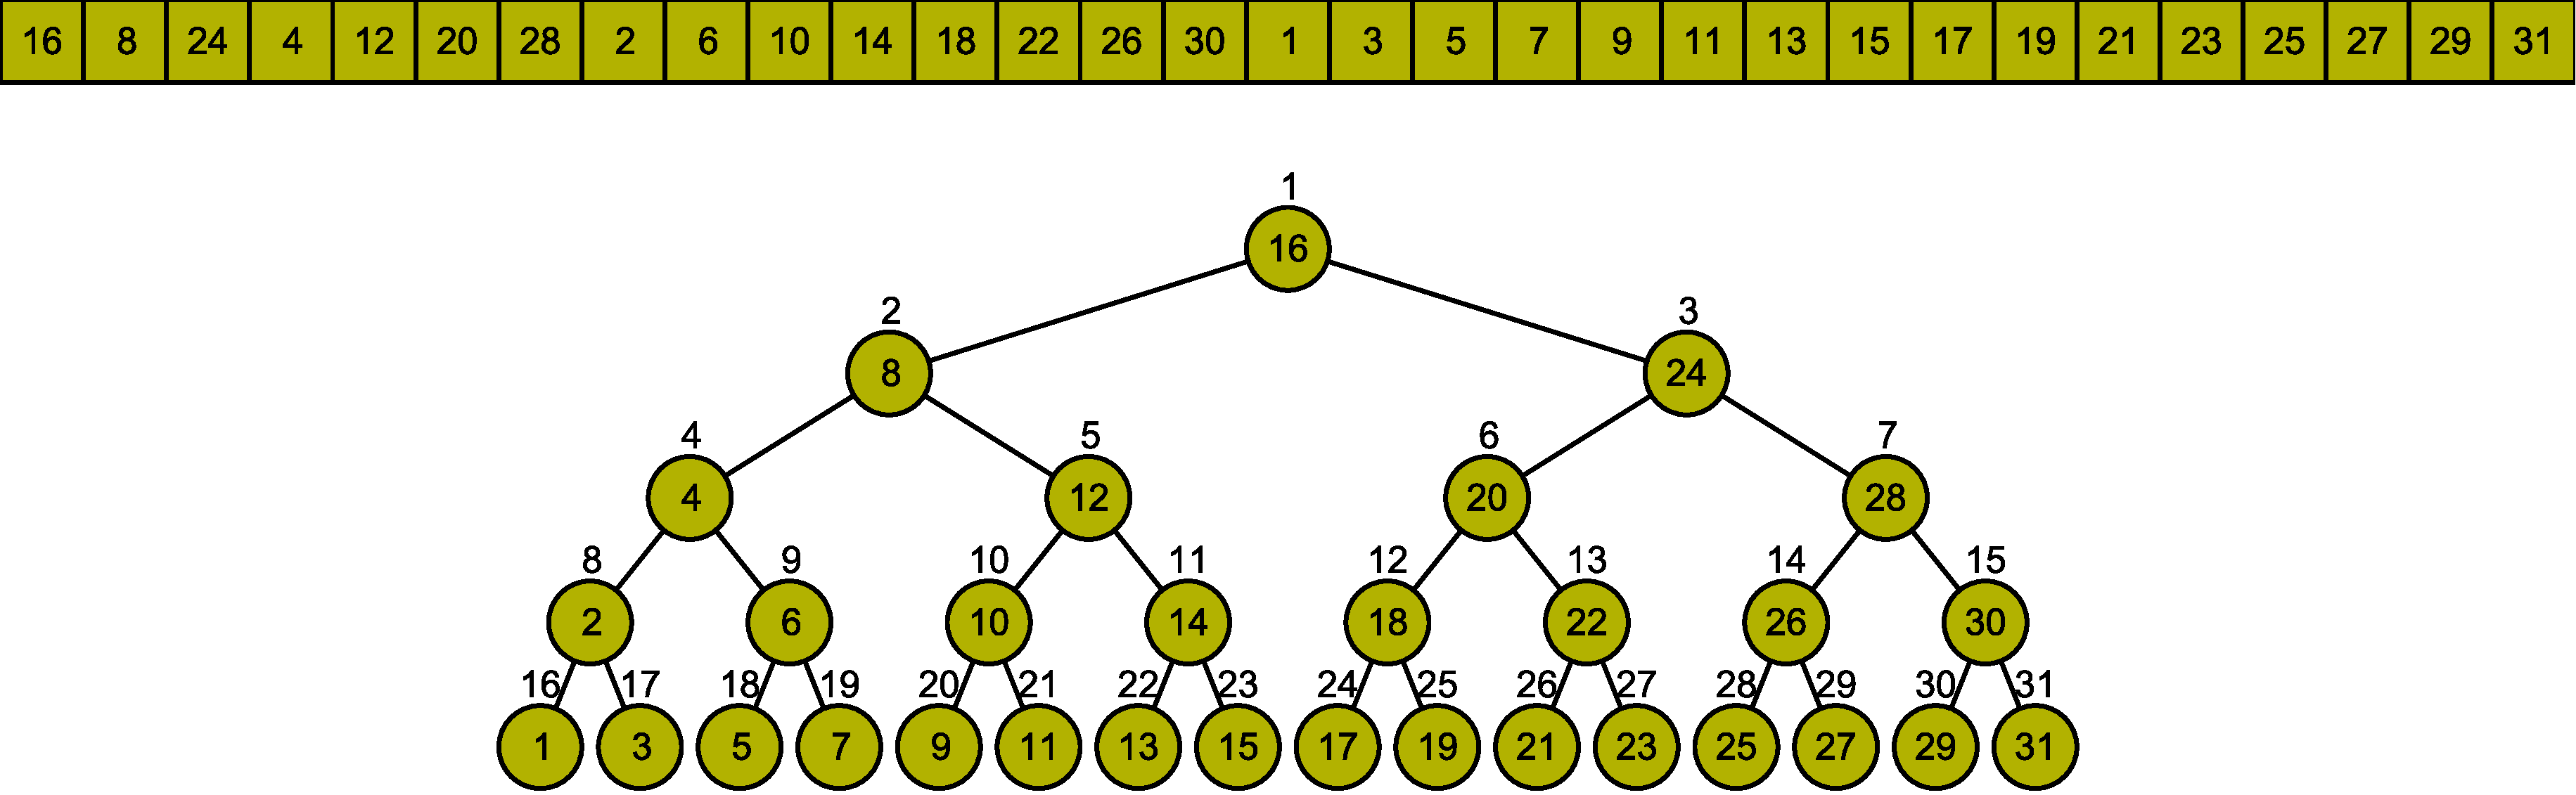
\includegraphics[width=\textwidth]{figures/screenshots/static_size_5_bfs.pdf}}
    \caption{Rozdiel medzi klasickým a \vEB usporiadaním na strome výšky 5.}
    \label{fig:ss_static_order}
\end{figure}

\subsection{Simulácia \cache}
Porovnanie týchto dvoch usporiadaní je rozšírené o simuláciu \cache. Užívateľ si môže zvoliť parametre cache - počet vrcholov $B$, ktoré sa zmestia do jedného bloku a počet blokov $\frac{M}{B}$ v \cache. Táto simulácia zároveň počíta počet prístupov k vrcholom pri vyhľadávaní a počet presunutých blokov do \cache. V najhoršom prípade by tieto dve čísla boli rovnaké (ak treba každý vrchol načítať osobitne) avšak pri \cache s blokmi veľkosti $B > 1$ a s \vEB usporiadaním dochádza k podstatnému zlepšeniu - ušetreniu počtu presunutých blokov.

\todo[inline]{screenshot}

Ako vizualizácia \cache slúži farba - vrcholy a položky poľa obsahujúce kľúče majú svetlejšiu farbu pozadia v prípade, že je daný blok v \cache a tmavšiu ak je mimo. V strome je vďaka tomu ľahko vidieť, ktorá časť je načítaná a je možné ňou prechádzať bez ďalších presunov. V prípade \vEB usporiadanie pôjde prevažne o časť podstromu aktuálne porovnávaného vrcholu, avšak pri klasickom usporiadaní to budú práve vrcholy mimo tohto podstromu, o ktorých už vieme, že nie sú pri vyhľadávaní potrebné.

\section{Usporiadané pole}
\todo[inline]{Layout, intro}
\subsection{Vkladanie}

\section{Dynamický strom}
\todo[inline]{Layout, intro}
\subsection{Vyhľadávanie}
\subsection{Vkladanie}

\section{Implementácia}
\todo[inline]{?}

%Visualization
%- intro
%- existing - none?
%- algvis history
%- implementation details
%  - cache simulation
%- list of structures
%  - static tree
%    - intro
%    - array order
%    - cache simulation
%    - order switching
%  - ordered file
%    - intro
%    - insert
%  - cobtree
%    - intro
%    - layout
%    - find
%    - insert
%- testovanie?
